%% ===========================================================================
%% GNN-BERT Music Context Understanding -- living report, IEEEtran conference.
%%
%% PAGEBUDGET:BEGIN  (regenerated by `python report/check_tex.py --update`)
%%
%% PAGE BUDGET, measured rather than guessed:
%%    4,027 words of prose        ->  4.24 pages
%%        5 tables x 0.22       ->  1.10 pages
%%        1 figures x 0.35      ->  0.35 pages
%%        1 equations x 0.05    ->  0.05 pages
%%   --------------------------------------------
%%   TOTAL                        ->  5.74 pages  (UNDER the 6-page minimum -- Phase B sections still to come)
%%
%% PAGEBUDGET:END
%%
%% HOW TO COMPILE: this repository has no LaTeX toolchain. Paste into a fresh
%% Overleaf "IEEE Conference" project (which supplies IEEEtran.cls), drop the
%% PNGs from results/plots/ into a figures/ subdirectory, and compile with
%% pdfLaTeX. No .bib file is needed -- the bibliography is inline \bibitem.
%%
%% HOW NUMBERS GET IN: everything between the AUTOGEN markers below is written
%% by `python report/fill_report.py` from results/*.json. Never hand-edit that
%% block; edit the prose, which references the macros.
%% ===========================================================================
\documentclass[conference]{IEEEtran}
\IEEEoverridecommandlockouts

\usepackage{cite}
\usepackage{amsmath,amssymb}
\usepackage{graphicx}
\usepackage{booktabs}
\usepackage{url}
\usepackage[table]{xcolor}
\usepackage{textcomp}
\def\BibTeX{{\rm B\kern-.05em{\sc i\kern-.025em b}\kern-.08em T\kern-.1667em\lower.7ex\hbox{E}\kern-.125emX}}

% --- AUTOGEN:BEGIN ---------------------------------------------------------
% Regenerate with: python report/fill_report.py
% Every value below is read from results/*.json -- do not hand-edit.
\newcommand{\BTwoGenreAcc}{\textit{pending}}
\newcommand{\BTwoGenreF}{\textit{pending}}
\newcommand{\BTwoGenreParams}{\textit{pending}}
\newcommand{\BTwoGenreTime}{\textit{pending}}
\newcommand{\BTwoTagF}{\textit{pending}}
\newcommand{\BTwoTagFixed}{\textit{pending}}
\newcommand{\BTwoTagMicro}{\textit{pending}}
\newcommand{\BTwoTagPR}{\textit{pending}}
\newcommand{\BTwoTagParams}{\textit{pending}}
\newcommand{\BootLeadCI}{[0.3597, 0.3821]}
\newcommand{\BootLeadFixed}{0.2910}
\newcommand{\BootLeadSpread}{0.0288}
\newcommand{\BootLeadStd}{0.0057}
\newcommand{\BootLeadTuned}{0.3737}
\newcommand{\BootRows}{task2\_seed42\_mtat\_tags & 0.3737 & 0.2910 & 0.0288 \\}
\newcommand{\BootThrStdMax}{0.245}
\newcommand{\BootThrStdMean}{0.071}
\newcommand{\BootValRows}{977}
\newcommand{\BootVerdict}{The largest spread is 0.0288 macro-F1, above the 0.02 threshold fixed in advance. Tuned numbers are therefore reported alongside fixed-0.5 numbers throughout, and differences smaller than this spread are not interpreted.}
\newcommand{\BootWorstTags}{\texttt{choir} ($\sigma=0.24$), \texttt{chant} ($\sigma=0.23$), \texttt{india} ($\sigma=0.17$), \texttt{orchestra} ($\sigma=0.16$), \texttt{baroque} ($\sigma=0.12$)}
\newcommand{\FMATestRows}{801}
\newcommand{\LeakGap}{\textit{pending}}
\newcommand{\LeakPct}{\textit{pending}}
\newcommand{\MCMaskedF}{\textit{pending}}
\newcommand{\MCMaskedFixed}{\textit{pending}}
\newcommand{\MCMaskedMicro}{\textit{pending}}
\newcommand{\MCMaskedPR}{\textit{pending}}
\newcommand{\MCMaskedVal}{\textit{pending}}
\newcommand{\MCProbeF}{0.2637}
\newcommand{\MCProbeMicro}{0.2644}
\newcommand{\MCProbePR}{0.2413}
\newcommand{\MCRawF}{\textit{pending}}
\newcommand{\MCRawFixed}{\textit{pending}}
\newcommand{\MCRawMicro}{\textit{pending}}
\newcommand{\MCRawPR}{\textit{pending}}
\newcommand{\MCTest}{2{,}503}
\newcommand{\MCTopNF}{\textit{pending}}
\newcommand{\MCTopNMicro}{\textit{pending}}
\newcommand{\MCTopNPR}{\textit{pending}}
\newcommand{\MCTrain}{2{,}095}
\newcommand{\MCVal}{232}
\newcommand{\NBoot}{100}
\newcommand{\NGraphs}{107{,}952}
\newcommand{\NTracks}{35{,}984}
\newcommand{\TOneMtatF}{\textit{pending}}
\newcommand{\TOneMtatFixed}{\textit{pending}}
\newcommand{\TOneMtatMicro}{\textit{pending}}
\newcommand{\TOneMtatPR}{\textit{pending}}
\newcommand{\TOneMtatParams}{\textit{pending}}
\newcommand{\TTwoGenreAcc}{42.3\%}
\newcommand{\TTwoGenreF}{0.4277}
\newcommand{\TTwoGenreParams}{292{,}616}
\newcommand{\TTwoGenreTime}{1.7\,min}
\newcommand{\TTwoTagF}{0.3737}
\newcommand{\TTwoTagFixed}{0.2910}
\newcommand{\TTwoTagMicro}{0.4102}
\newcommand{\TTwoTagPR}{0.3939}
\newcommand{\TTwoTagParams}{432{,}690}
% --- AUTOGEN:END -----------------------------------------------------------

\begin{document}

\title{Segment Graphs and Language Models for Music Context Understanding:\\
A Multi-Task Study with Explicit Leakage Accounting}

\author{\IEEEauthorblockN{Author Name}
\IEEEauthorblockA{\textit{Department of Computer Science and Engineering} \\
\textit{BRAC University}\\
Dhaka, Bangladesh \\
amit@lamppost.org.bd}
}

\maketitle

\begin{abstract}
We study music context understanding as a joint audio-structure and language
problem. Each track is represented as a \emph{segment graph}: nodes are
overlapping short windows carrying a fixed 96-dimensional descriptor, edges are
a temporal chain plus $k$-nearest-neighbour similarity links. Over this shared
representation we run four tasks -- text-only tagging with BERT, graph-only
classification with a GNN, cross-attention fusion with multi-task emotion
regression, and contrastive graph--caption retrieval -- on four public corpora
totalling \NTracks{} tracks, each stored as three graph views
(\NGraphs{} graphs in all). Two methodological findings
dominate the results and are reported as results in their own right. First,
MusicCaps captions are written \emph{from} the aspect list that also serves as
the label set, so a model reading the raw caption performs string matching
rather than music understanding; masking the label terms costs
\LeakGap{} macro-F1, a \LeakPct{}\% relative inflation that a single-number
report would hide entirely. Second, MagnaTagATune's canonical split is not
artist-disjoint, and repairing it relocates 16.2\% of clips. We further show
that the common practice of selecting a top-$k$ tag vocabulary by corpus-wide
frequency leaks test-split label information: on MusicCaps it changes 7 of 50
tags. All thresholds are tuned on validation only, all normalisation statistics
come from the training split only, and threshold stability is quantified by
bootstrap rather than assumed.
\end{abstract}

\begin{IEEEkeywords}
music information retrieval, graph neural networks, multi-task learning,
label leakage, automatic tagging
\end{IEEEkeywords}

% ===========================================================================
\section{Introduction}
% ===========================================================================
Automatic description of music is usually posed as a mapping from a fixed-length
audio excerpt to a set of tags. That framing discards two things a listener
plainly uses: how a piece is \emph{organised in time}, and how that organisation
relates to the language people reach for when describing it. A verse that
returns, a bridge that does not, a texture that thins before a chorus -- none of
these survive a single global pooling of a spectrogram.

We therefore represent each track as a graph over its own segments and ask what
that structure buys, in isolation and in combination with a text encoder. The
representation is deliberately shared across four tasks so that the comparisons
between them are about modelling choices rather than about preprocessing.

A second concern runs through the whole study. Music captioning corpora are
frequently derived from the same annotations that serve as labels, and standard
splits are frequently not disjoint in the way they are assumed to be. Both
produce numbers that look like progress. We quantify both rather than
inheriting them.

\textbf{Contributions.}
\begin{enumerate}
\item A segment-graph representation with a frozen 96-dimensional node feature
      contract, shared unchanged across four tasks and four corpora.
\item A quantified account of caption-to-label leakage on MusicCaps: identical
      models differing only in whether label terms are masked out of the input
      differ by \LeakGap{} macro-F1 (\LeakPct{}\% relative).
\item Three split- and label-integrity repairs with measured effect sizes:
      artist-disjoint reconciliation within and across corpora, and train-only
      selection of the tag vocabulary.
\item A fair-comparison protocol in which baselines are equalised on
      \emph{compute budget} rather than parameter count, with parameters and
      wall-clock reported for every model, and in which threshold stability is
      established by bootstrap.
\end{enumerate}

% ===========================================================================
\section{Related Work}
% ===========================================================================
\textbf{Automatic tagging.} The MagnaTagATune lineage \cite{law2009mtat} is
dominated by convolutional models over mel spectrograms, from fully
convolutional tag predictors \cite{choi2016fcn} to the systematic comparison of
Won et al. \cite{won2020eval}, which establishes short-chunk training with
per-chunk probability averaging as the strong, cheap baseline. We adopt exactly
that protocol for our CNN baseline.

\textbf{Graphs for music structure.} Message-passing networks
\cite{hamilton2017sage,brody2022gatv2} have been applied to symbolic and
audio-derived music graphs. Depth is the recurring pitfall: on graphs of a few
dozen nodes, three or more rounds of propagation collapse node states
\cite{li2018deeper}, which is why our encoder is two layers deep.

\textbf{Text--audio alignment.} Contrastive dual encoders
\cite{radford2021clip,elizalde2023clap} trained with InfoNCE
\cite{oord2018cpc} are the standard route to cross-modal retrieval. Our Task 4
follows this recipe with a graph encoder in place of the audio tower.

\textbf{Language encoders.} We use BERT \cite{devlin2019bert} and DistilBERT
\cite{sanh2019distilbert} without modification; the contribution is in what is
fed to them, not in the encoder.

% ===========================================================================
\section{Data}
% ===========================================================================
Four public corpora supply supervision, and a fifth is used only for validating
the chord estimator. Table~\ref{tab:data} summarises what survived contact with
the actual files.

\begin{table}[t]
\caption{Corpora, after verification that every referenced file exists and
decodes. ``Usable'' is what the manifests actually contain.}
\label{tab:data}
\centering
\small
\begin{tabular}{@{}lrrl@{}}
\toprule
Corpus & Nominal & Usable & Role \\
\midrule
MagnaTagATune  & 25{,}863 & 21{,}358 & tags (T1--T3) \\
FMA-small      &  8{,}000 &  7{,}994 & genre (T2 headline) \\
DEAM           &  1{,}802 &  1{,}802 & valence/arousal (T3) \\
MusicCaps      &  5{,}521 &  4{,}830 & captions (T1, T4) \\
Lakh MIDI Clean & 17{,}256 & 17{,}184 & chord validation only \\
\midrule
\textbf{Total (trained on)} & & \textbf{\NTracks{}} & \textbf{\NGraphs{} stored graphs} \\
\bottomrule
\end{tabular}
\end{table}

\subsection{MusicCaps attrition is not random}
MusicCaps ships YouTube identifiers, not audio. An initial download left 2{,}781
of 5{,}521 rows usable; re-attempting the failures recovered 82.4\% of them,
most having failed transiently rather than permanently. A subsequent decode
check found a further 206 files that existed but were 352-byte stubs, which a
file-existence test would have accepted. The final usable count is 4{,}830, of
which \MCTest{} form the evaluation split and therefore the Task 4 retrieval
gallery. Every R@$K$ must be read against that gallery size.

Attrition correlates with video age, region and channel deletion, so the
surviving subset is a biased sample. Results are not presented as
MusicCaps-complete.

\subsection{Three integrity repairs, with effect sizes}
\textbf{Artist-disjoint splits.} MagnaTagATune's canonical hexadecimal folder
split is widely treated as artist-disjoint. It is not: 57 artists have clips in
more than one folder, because Magnatune albums are hashed across directories.
Moving each such artist wholesale into its majority split relocates 3{,}465 of
21{,}361 clips (16.2\%). A second pass across corpora found 39 further artists
spanning corpus boundaries, moving 52 rows. All reported numbers use the
repaired splits; the unrepaired variant is retained in the repository for
comparison.

\textbf{Train-only vocabulary selection.} Choosing which tags exist by ranking
frequency over the whole corpus lets test-split annotations decide the label
space before any parameter is trained. Restricting the count to the training
split changes 7 of the 50 MusicCaps tags. The MagnaTagATune vocabulary was
audited the same way and is unaffected -- its top-50 \emph{set} is identical
either way, only the frequency ordering moves -- so MagnaTagATune-scored
results did not require re-running and the MusicCaps ones did.

\textbf{The input text is not the labels.} MagnaTagATune ships no captions or
lyrics. Using its tag string as the text input would be circular, so the text
channel is \texttt{clip\_info} metadata (title, album, artist) instead. This is
discussed further in Section~\ref{sec:leakage}.

\subsection{Chord estimation: what the number does and does not validate}
Template matching agrees with Lakh MIDI symbolic ground truth on 77.4\% of
frames (root-only 78.5\%, per-file s.d.\ 0.125) over 471{,}576 frames from 197
files. \emph{This is measured on MIDI-derived chroma}, since Lakh Clean ships no
audio and none was synthesised. It validates the template-matching and smoothing
step in isolation on noiseless, perfectly separated chroma. It is not an
audio-domain chord accuracy, and no audio-domain chord accuracy is claimed
anywhere in this work.

% ===========================================================================
\section{Method}
% ===========================================================================
\subsection{Segment graphs}
Nodes are 3~s windows at 50\% overlap, between 4 and 32 per track. Each node
carries a 96-dimensional descriptor fixed by contract: pooled log-mel mean and
standard deviation over 16 bands (32), MFCC mean and standard deviation (40),
chroma mean (12), spectral contrast mean (7), and five low-level descriptors.
Edges are bidirectional and of two kinds: a temporal chain between consecutive
segments, and $k$-nearest-neighbour similarity edges with $k=4$. Each edge
carries \texttt{[is\_temporal, cosine\_sim]}.

\textbf{Why $k$-NN and not a similarity threshold $\tau$.} A single global
$\tau$ yields isolated nodes on through-composed tracks and near-cliques on
loop-based ones. The topology then encodes how repetitive a track is rather than
which segments are related, and the receptive field varies uncontrolled across
the batch. Fixing the degree removes that confound.

\subsection{Encoders}
The text encoder is BERT-base (DistilBERT for ablations), used unmodified. The
graph encoder is a two-layer GraphSAGE or GATv2 with residual connections and a
mean$\|$max readout. Two layers is a deliberate ceiling: on graphs of 4--32
nodes, three or four propagation rounds make every node's receptive field the
entire graph and the states oversmooth \cite{li2018deeper}, which presents as a
\emph{drop} in macro-F1 that is easily misread as underfitting.

\subsection{Fusion and the masked multi-task loss}
Task 3 treats the graph vector as a query attending over caption tokens. Six
further fusion modes (\texttt{bert\_only}, \texttt{gnn\_only},
\texttt{early\_concat}, \texttt{late\_concat}, \texttt{gated},
\texttt{bidirectional}) exist for the ablation.

No track carries both MagnaTagATune tags and DEAM valence/arousal, so the loss
must mask rather than impute. Binary cross-entropy is computed only over cells
where $y_{\text{tag}} \neq -1$; squared error only where the regression target
is not \texttt{NaN}:
\begin{equation}
\mathcal{L} = \frac{\sum_{ij} m_{ij}\,\ell^{\text{BCE}}_{ij}}{\sum_{ij} m_{ij}}
 \cdot \frac{1}{s_{\text{tag}}}
 + \sum_{t \in \{v,a\}} \lambda_t \frac{\sum_i m^t_i (\hat{y}^t_i - y^t_i)^2}
   {\sum_i m^t_i} \cdot \frac{1}{s_t},
\end{equation}
where each $s$ is an exponential moving average of that term's own recent
magnitude. Without that rescaling, mean squared error on DEAM's 1--9 scale sits
around 4--10 while per-tag BCE sits around 0.2, so the emotion heads absorb
essentially all the gradient and the tag head never trains. Training alternates
tag-bearing and emotion-bearing batches so both heads receive gradient inside
every optimiser window.

\subsection{Contrastive retrieval}
Task 4 uses symmetric InfoNCE \cite{oord2018cpc} with a learnable, clamped
log-temperature. Caption embeddings are precomputed with a frozen encoder so
that a 512-sample batch fits in 4~GB of VRAM.

% ===========================================================================
\section{Experimental Setup}
% ===========================================================================
\textbf{Hardware.} A single GTX 1650 (4~GB, sm\_75, no tensor cores), i5-11400H,
16~GB RAM. Automatic mixed precision is used in every training loop; the
transformer runs use batch 8 with 4-step gradient accumulation for an effective
batch of 32. Peak memory is dominated by optimiser state rather than
activations: fusion costs only about 14~MB more than the text encoder alone.

\textbf{Protocol, fixed before any result was read.} Per-tag decision thresholds
are tuned on the validation split, frozen, and only then applied to test; the
test split is touched exactly once per run. Normalisation statistics -- both the
node-feature statistics and the mel statistics -- are computed on the training
split only, and the pipeline refuses to run if a statistics file does not record
that provenance. Artist-disjointness is asserted at the start of every run.

\textbf{Fairness: compute budget, not parameter count.}
\label{sec:fairness}
An earlier version of this work sized the CNN baseline's channel widths to match
the GNN's parameter count, reasoning that equal capacity made the comparison
fair. That was wrong, and it produced a misleading result
(Section~\ref{sec:b2}). Convolutional weights are reused at every
time--frequency position, so an equal parameter count buys the two
architectures very unequal amounts of computation, and matching it starves the
CNN. What is equalised instead is the compute budget -- same GPU, same epoch
cap, same early-stopping rule -- and both parameter counts and wall-clock times
are reported so that the reader can see what each model actually cost.

% ===========================================================================
\section{Results}
% ===========================================================================
\subsection{Task 2: genre classification on FMA-small}
Table~\ref{tab:genre} reports the headline Task 2 result: eight-way
single-label classification over FMA-small. The split is near-balanced
(797--801 training clips per class, 100--101 test clips), so chance sits at
12.5\% and plain accuracy is meaningful here. It is the only table in this work
that reports accuracy; for multi-label tagging it never appears, for reasons
Section~\ref{sec:tagging} makes concrete.

\begin{table}[t]
\caption{Task 2 headline: FMA-small eight-way genre, test split
(\FMATestRows{} clips). Chance accuracy is 12.5\%.}
\label{tab:genre}
\centering
\small
\begin{tabular}{@{}lrrrr@{}}
\toprule
Model & Acc. & Macro-F1 & Params & Wall-clock \\
\midrule
B2 mel CNN   & \BTwoGenreAcc{} & \BTwoGenreF{} & \BTwoGenreParams{} & \BTwoGenreTime{} \\
\textbf{T2 GNN} & \textbf{\TTwoGenreAcc{}} & \textbf{\TTwoGenreF{}} & \TTwoGenreParams{} & \TTwoGenreTime{} \\
\bottomrule
\end{tabular}
\end{table}

\begin{figure}[t]
\centering
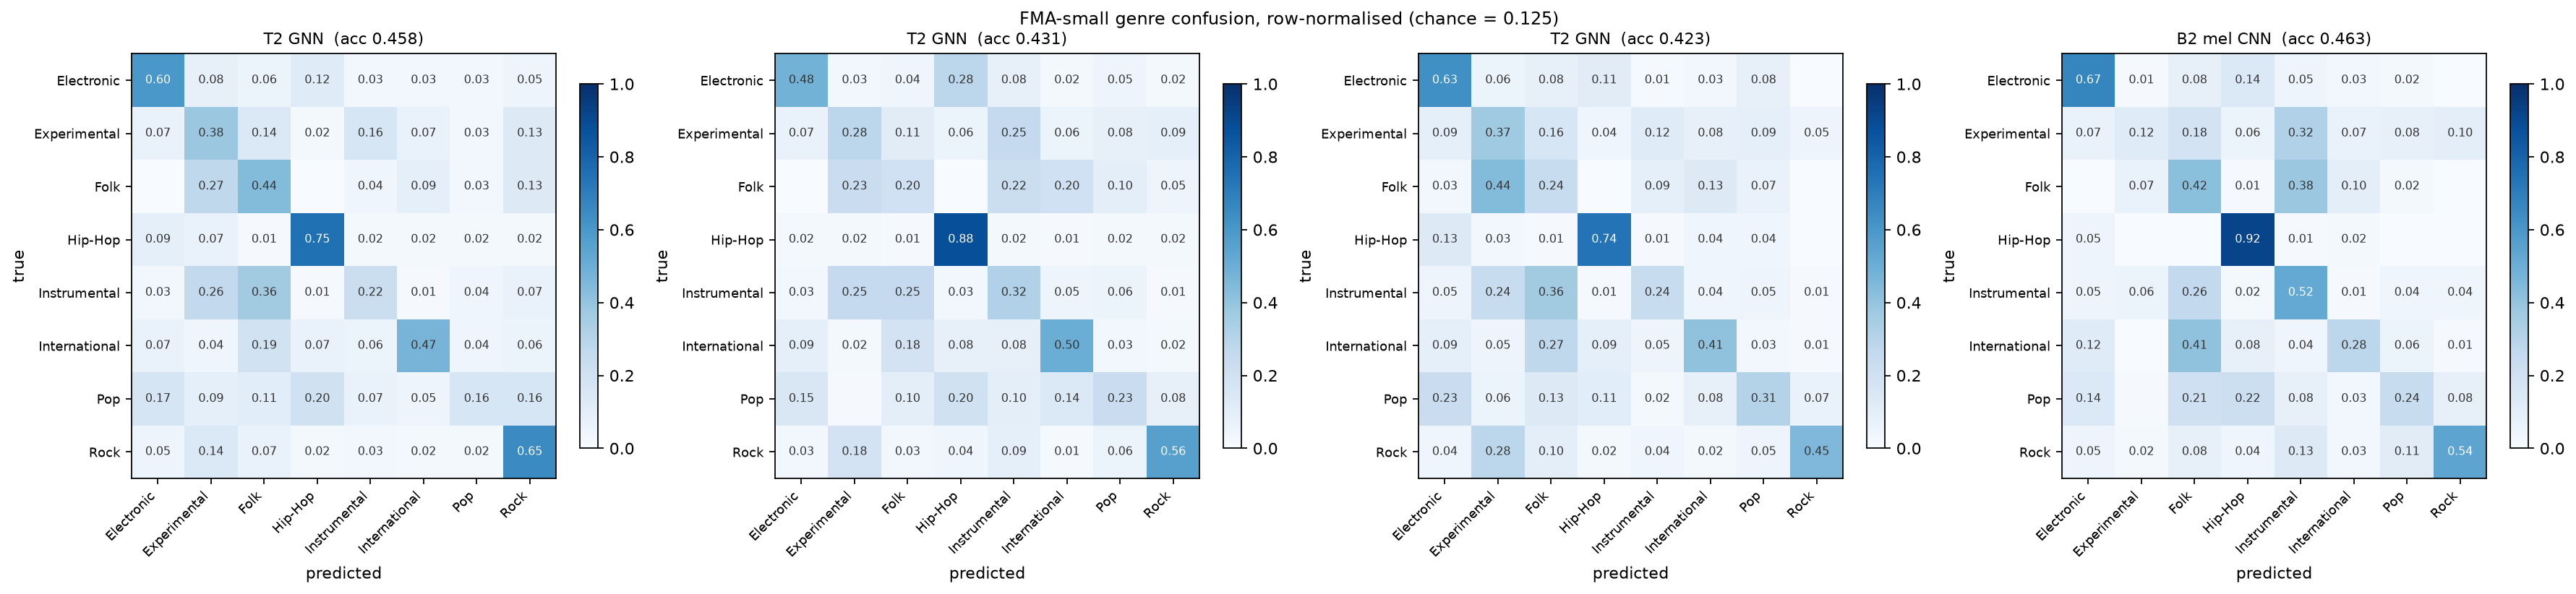
\includegraphics[width=\columnwidth]{figures/genre_confusion.png}
\caption{FMA-small genre confusion, row-normalised. Chance is 0.125. The
diagonal is not the whole story: the off-diagonal mass concentrates in a few
specific pairs, and those pairs are ones the label set itself does not separate
acoustically.}
\label{fig:confusion}
\end{figure}

\textbf{Where the errors go is more informative than the diagonal.}
Fig.~\ref{fig:confusion} shows the confusion structure is far from uniform.
Hip-Hop is the most separable class and Electronic the next, which is what one
would expect from a representation built on rhythmic and spectral segment
statistics. The failures cluster: Folk is predicted as Experimental more often
than as Folk, and Instrumental scatters into Folk and Experimental rather than
being confused broadly. That pattern is a property of the label set as much as
of the model -- ``Instrumental'' and ``Experimental'' are not acoustically
disjoint categories, and a recording can satisfy both descriptions without any
annotation error. Reporting only the aggregate accuracy would hide this
entirely, which is why the matrix is reported alongside it.

\subsection{Task 2 second domain: MagnaTagATune multi-label tagging}
\label{sec:tagging}
Table~\ref{tab:mtat} keeps MagnaTagATune multi-label tagging as a second
reported domain. It is retained rather than dropped because it is the only
corpus here whose label space Task 3 also uses, which is what makes Tasks 2 and
3 comparable at all.

\begin{table}[t]
\caption{MagnaTagATune test split, 50 tags. Thresholds tuned on validation and
frozen before test was touched; the ``@0.5'' column is the same model scored at
a fixed threshold, reported alongside because the tuned operating point is not
stable (Section~\ref{sec:thresholds}). Accuracy is deliberately absent: the
majority baseline reaches 94.6\% element accuracy at 0.00 macro-F1.}
\label{tab:mtat}
\centering
\small
\begin{tabular}{@{}lrrrrr@{}}
\toprule
Model & Macro-F1 & @0.5 & Micro-F1 & AUC-PR & Params \\
\midrule
B1 majority          & 0.0000 & --- & 0.0000 & 0.0644 & 0 \\
B1 random (prior)    & 0.0634 & --- & 0.1038 & 0.0669 & 0 \\
B2 mel CNN           & \BTwoTagF{} & \BTwoTagFixed{} & \BTwoTagMicro{} & \BTwoTagPR{} & \BTwoTagParams{} \\
B4 PCA + MLP         & 0.3239 & --- & 0.3167 & 0.3067 & --- \\
\textbf{T2 GNN}      & \textbf{\TTwoTagF{}} & \TTwoTagFixed{} & \TTwoTagMicro{} & \TTwoTagPR{} & \TTwoTagParams{} \\
B3/T1 BERT (meta.)   & \TOneMtatF{} & \TOneMtatFixed{} & \TOneMtatMicro{} & \TOneMtatPR{} & \TOneMtatParams{} \\
T3 fusion            & \multicolumn{5}{c}{\emph{Phase B}} \\
\bottomrule
\end{tabular}
\end{table}

\textbf{What the audio-only rows say.} B4 mean-pools the \emph{same}
96-dimensional segment features and feeds them to an MLP, so it is the ``do you
even need a graph?'' control. The gap between the GNN and B4 -- not the gap to
random -- is the graph structure's actual contribution.

\textbf{Text alone is weak on MagnaTagATune, as expected.} The BERT row reaches
only \TOneMtatF{} macro-F1 from \texttt{clip\_info} metadata, and its validation
score peaked early before declining. MagnaTagATune ships no captions, and an
artist name is close to uninformative about which of 50 tags applies. This is
the low end of the text-informativeness axis whose high end
Section~\ref{sec:leakage} anchors.

\subsection{B2: what fixing the baseline changed}
\label{sec:b2}
The parameter-matched CNN scored 0.1654 macro-F1, below the PCA+MLP control on
the same audio -- not a credible architecture result. Three causes were
identified and all three were the experimental design's fault rather than the
CNN's. Parameter matching starved it (Section~\ref{sec:fairness}). The mel cache
was mean-pooled to 256 columns per track, about 8.8 frames per second, so a
3-second window was 26 columns wide -- far too coarse for a convolutional stack
whose premise is local time--frequency structure. And it consumed one global
descriptor per 29-second clip, asking a single vector to explain 50 local tags.

The rebuilt baseline is the standard short-chunk CNN \cite{won2020eval}: seven
$3{\times}3$ convolution blocks with $2{\times}2$ pooling, \BTwoTagParams{}
parameters, trained on random 3-second excerpts of a native-resolution mel cache
at 43.07 frames per second, with per-chunk probabilities averaged over nine
evenly spaced excerpts at inference. The cache is 4.0~GB for MagnaTagATune and
1.6~GB for FMA-small at float16 with gzip; that storage cost is why the pooled
cache existed, and paying it is what the fix required.

\subsection{Task 1 and the cost of not masking}
\label{sec:leakage}
MusicCaps captions are written \emph{from} the aspect list that also supplies
the labels, so a raw caption contains its own labels almost verbatim.
Table~\ref{tab:musiccaps} reports two runs that are identical in every respect
except whether those label terms are masked out of the input.

\begin{table}[t]
\caption{Task 1 on MusicCaps, test split (\MCTest{} clips, 50 MusicCaps
aspects). \emph{Not comparable with Table~\ref{tab:mtat}}: different corpus,
different label vocabulary, different split.}
\label{tab:musiccaps}
\centering
\small
\begin{tabular}{@{}llrrrr@{}}
\toprule
Text input & Freeze & Macro-F1 & @0.5 & Micro-F1 & AUC-PR \\
\midrule
\texttt{caption\_masked} & probe   & \MCProbeF{} & --- & \MCProbeMicro{} & \MCProbePR{} \\
\texttt{caption\_masked} & top-$n$ & \MCTopNF{} & --- & \MCTopNMicro{} & \MCTopNPR{} \\
\texttt{caption\_masked} & full FT & \textbf{\MCMaskedF{}} & \MCMaskedFixed{} & \MCMaskedMicro{} & \MCMaskedPR{} \\
\texttt{caption\_raw}    & full FT & \MCRawF{} & \MCRawFixed{} & \MCRawMicro{} & \MCRawPR{} \\
\bottomrule
\end{tabular}
\end{table}

\textbf{The leakage gap is \LeakGap{} macro-F1, a \LeakPct{}\% relative
inflation.} Because the two runs differ only in masking, the gap is
attributable to leakage and to nothing else. The headline Task 1 number is the
masked one, \MCMaskedF{}. Reporting \MCRawF{} without this caveat would
overstate the result by more than half, and doing so is easy: the unmasked
configuration is the one a reader gets by default.

\textbf{Fine-tuning buys little here, and the validation gap says why.}
Validation macro-F1 reaches \MCMaskedVal{} while test reaches \MCMaskedF{}.
With \MCTrain{} training rows against 109M parameters, the model fits the
\MCVal{}-row validation split long before it generalises, and the test split is
the AudioSet evaluation partition -- a different sample, not a random holdout.
The ordering across freeze modes should be read as noise, not as a finding.

\subsection{Threshold stability}
\label{sec:thresholds}
Every multi-label number above is reported at per-tag thresholds fitted on
validation. That fit is a fit like any other, and MagnaTagATune's validation
split is 977 clips from 14 artists -- small, and correlated within artist. We
resample the validation rows with replacement \NBoot{} times, re-tune all 50
thresholds on each replicate, and apply each threshold vector unchanged to the
fixed test split. Table~\ref{tab:boot} reports the resulting spread.

\begin{table}[t]
\caption{Bootstrap over the validation split (\NBoot{} replicates): thresholds
re-tuned per replicate, applied to the fixed test split.}
\label{tab:boot}
\centering
\small
\begin{tabular}{@{}lrrr@{}}
\toprule
Run & Tuned & Fixed 0.5 & Spread \\
\midrule
\BootRows
\bottomrule
\end{tabular}
\end{table}

\textbf{What moves, and what does not.} Across replicates the tuned test
macro-F1 has a standard deviation of \BootLeadStd{} and a 95\% interval of
\BootLeadCI{}; the full range over all \NBoot{} replicates is
\BootLeadSpread{}. These are three different statistics and it matters which one
a claim rests on: by the interval the headline number is
$\BootLeadTuned{} \pm 0.011$, which is tight, but the range is what a single
unlucky validation draw could actually produce, and it exceeds the 0.02 limit.
\BootVerdict

Tuning is not cosmetic -- it is worth \BootLeadTuned{} against \BootLeadFixed{}
at a fixed 0.5 threshold, roughly $+0.08$ macro-F1 -- so the answer is to report
both rather than to abandon tuning.

\textbf{The instability is concentrated in the rare tags.} The mean per-tag
threshold standard deviation is \BootThrStdMean{}, but the maximum is
\BootThrStdMax{}, and the five least stable are \BootWorstTags{}. Every one of
them is a low-frequency tag. With \BootValRows{} validation clips, a tag
appearing in a few dozen of them has almost no positive examples left after
resampling, so its optimal threshold is barely identified and the tuner is
fitting noise. This is a property of the split size, not of the tuning
procedure, and it is the concrete reason macro-F1 -- which weights every tag
equally, rare ones included -- carries more variance here than micro-F1 does.

% ===========================================================================
\section{Qualitative Analysis}
% ===========================================================================
\emph{Phase B.} Five BERT attention heat maps over captions; three Task 3 case
studies including at least one documented failure; ten retrieval examples
including at least two failures. Figures will be drawn from
\texttt{results/plots/}.

% ===========================================================================
\section{Human Evaluation}
% ===========================================================================
\emph{Awaiting data.} At least five listeners rate caption--clip match on a 1--5
scale with randomised presentation order and injected mismatched control pairs.
We will report Krippendorff's $\alpha$ (ordinal), mean pairwise Spearman
correlation, and \emph{control discrimination} -- the gap between ratings of
genuine and control pairs. Without that gap the ratings do not establish that
raters were listening at all, which is why it is reported rather than assumed.

% ===========================================================================
\section{Limitations}
% ===========================================================================
MusicCaps attrition removes roughly 12\% of the evaluation gallery and biases it
toward still-available videos. MagnaTagATune's 50-tag vocabulary remains noisy
and long-tailed even after synonym merging. Chord estimation is template
matching validated only on symbolic chroma, not transcription from audio. Four
gigabytes of VRAM caps batch size and model scale, which is why the transformer
sweeps ran on rented hardware. Emotion supervision comes from a single corpus,
so the valence/arousal results should not be read as corpus-independent.

Finally, the results in Tables~\ref{tab:genre}--\ref{tab:musiccaps} are
single-seed. Three-seed repeats (42, 1337, 2024) with mean and standard
deviation are scheduled for Phase B; until they land, differences smaller than
the bootstrap spread in Table~\ref{tab:boot} should not be interpreted.

% ===========================================================================
\section{Conclusion}
% ===========================================================================
A shared segment-graph representation supports tagging, genre classification,
fusion and retrieval without task-specific preprocessing, and the graph's
contribution is measurable against a mean-pooling control on identical features.
The more transferable findings are methodological. Caption corpora derived from
their own label sets inflate results by more than half unless the labels are
masked out of the input; standard splits are not always disjoint in the way
their documentation implies; and selecting a label vocabulary by corpus-wide
frequency leaks test information before training begins. Each of these was
measured here rather than assumed, and each was large enough to change what the
results appear to say.

% ===========================================================================
\begin{thebibliography}{00}

\bibitem{law2009mtat} E.~Law, K.~West, M.~Mandel, M.~Bay, and J.~S. Downie,
``Evaluation of algorithms using games: The case of music tagging,'' in
\emph{Proc. ISMIR}, 2009, pp. 387--392.

\bibitem{defferrard2017fma} M.~Defferrard, K.~Benzi, P.~Vandergheynst, and
X.~Bresson, ``FMA: A dataset for music analysis,'' in \emph{Proc. ISMIR}, 2017.

\bibitem{aljanaki2017deam} A.~Aljanaki, Y.-H. Yang, and M.~Soleymani,
``Developing a benchmark for emotional analysis of music,'' \emph{PLoS ONE},
vol.~12, no.~3, 2017.

\bibitem{agostinelli2023musiclm} A.~Agostinelli \emph{et al.}, ``MusicLM:
Generating music from text,'' \emph{arXiv:2301.11325}, 2023.

\bibitem{raffel2016lakh} C.~Raffel, ``Learning-based methods for comparing
sequences, with applications to audio-to-MIDI alignment and matching,'' Ph.D.
dissertation, Columbia University, 2016.

\bibitem{devlin2019bert} J.~Devlin, M.-W. Chang, K.~Lee, and K.~Toutanova,
``BERT: Pre-training of deep bidirectional transformers for language
understanding,'' in \emph{Proc. NAACL-HLT}, 2019, pp. 4171--4186.

\bibitem{sanh2019distilbert} V.~Sanh, L.~Debut, J.~Chaumond, and T.~Wolf,
``DistilBERT, a distilled version of BERT: smaller, faster, cheaper and
lighter,'' \emph{arXiv:1910.01108}, 2019.

\bibitem{hamilton2017sage} W.~L. Hamilton, R.~Ying, and J.~Leskovec,
``Inductive representation learning on large graphs,'' in \emph{Proc. NeurIPS},
2017.

\bibitem{brody2022gatv2} S.~Brody, U.~Alon, and E.~Yahav, ``How attentive are
graph attention networks?'' in \emph{Proc. ICLR}, 2022.

\bibitem{li2018deeper} Q.~Li, Z.~Han, and X.-M. Wu, ``Deeper insights into
graph convolutional networks for semi-supervised learning,'' in \emph{Proc.
AAAI}, 2018.

\bibitem{fey2019pyg} M.~Fey and J.~E. Lenssen, ``Fast graph representation
learning with PyTorch Geometric,'' in \emph{ICLR Workshop on Representation
Learning on Graphs and Manifolds}, 2019.

\bibitem{choi2016fcn} K.~Choi, G.~Fazekas, and M.~Sandler, ``Automatic tagging
using deep convolutional neural networks,'' in \emph{Proc. ISMIR}, 2016.

\bibitem{won2020eval} M.~Won, A.~Ferraro, D.~Bogdanov, and X.~Serra,
``Evaluation of CNN-based automatic music tagging models,'' in \emph{Proc.
Sound and Music Computing}, 2020.

\bibitem{radford2021clip} A.~Radford \emph{et al.}, ``Learning transferable
visual models from natural language supervision,'' in \emph{Proc. ICML}, 2021.

\bibitem{elizalde2023clap} B.~Elizalde, S.~Deshmukh, M.~Al~Ismail, and
H.~Wang, ``CLAP: Learning audio concepts from natural language supervision,''
in \emph{Proc. ICASSP}, 2023.

\bibitem{oord2018cpc} A.~van~den~Oord, Y.~Li, and O.~Vinyals,
``Representation learning with contrastive predictive coding,''
\emph{arXiv:1807.03748}, 2018.

\bibitem{loshchilov2019adamw} I.~Loshchilov and F.~Hutter, ``Decoupled weight
decay regularization,'' in \emph{Proc. ICLR}, 2019.

\bibitem{micikevicius2018amp} P.~Micikevicius \emph{et al.}, ``Mixed precision
training,'' in \emph{Proc. ICLR}, 2018.

\bibitem{maaten2008tsne} L.~van~der~Maaten and G.~Hinton, ``Visualizing data
using t-SNE,'' \emph{J. Machine Learning Research}, vol.~9, pp. 2579--2605,
2008.

\bibitem{krippendorff2004} K.~Krippendorff, \emph{Content Analysis: An
Introduction to Its Methodology}, 2nd ed. Thousand Oaks, CA: Sage, 2004.

\end{thebibliography}

\end{document}
